\paragraph{External Sorting using Index}

\paragraph{Basic concepts: B+ Trees}
\begin{itemize}
\item Each node in the tree occupies a page
\item Entries in non-leave nodes → called index entries: \\
  {\color{red} <key value, page\_id>}
\item Entries in leaf nodes → called data entries
  \begin{itemize}
  \item either containing actual data (direct index)
  \item or pointer to them (indirect index)
  \end{itemize}
\end{itemize}

\paragraph{Using B+ Trees for Sorting}

\textbf{Scenario:}
\begin{itemize}
\item Table to be sorted has B+ tree index on sorting column(s)
\end{itemize}

\textbf{Idea:}
\begin{itemize}
\item Can retrieve records in order by traversing leaf pages
\end{itemize}

\begin{itemize}
\item \textbf{Cost:} root to the left-most leaf, then retrieve all
  leaf pages (direct index)
\item if indirect index is used? Additional cost of retrieving
  data records: each page fetched just once
\end{itemize}

⇒ Always better than external sorting!


\begin{itemize}
\item If Unclustered (and indirect) index:
  \begin{itemize}
  \item Each data entry contains pointer to a data record
  \item Data records are not stored in the sorted order of the index
  \end{itemize}

\item In general, \textbf{one I/O per data record!}
\end{itemize}


\section{Implementation of Relational Operators}

\paragraph{Translating SQL Query to Relational Operators}

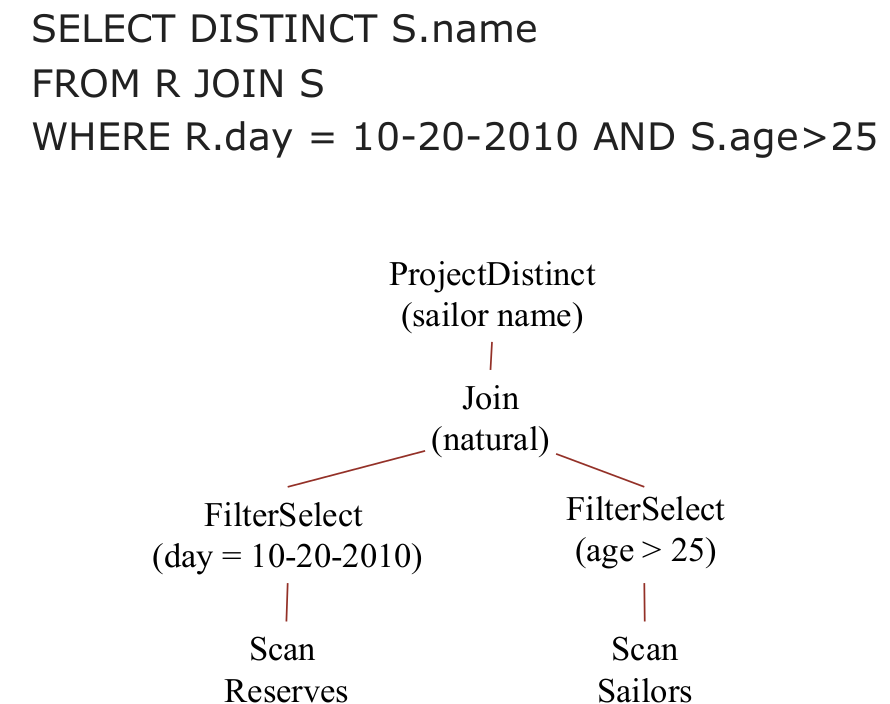
\includegraphics[scale=0.2]{graphics/sql-to-relational-op.png}


\paragraph{Relational Operator Implementation}
Implementing relational operators is challenging because:

\begin{itemize}
\item Relational queries are declarative
  \begin{itemize}
  \item There is no efficient predefined strategy
  \end{itemize}

\item The data sets are typically very large
\end{itemize}

Different Relational operators:
\begin{itemize}
\item Select
\item Project
\item Join
\item Set operations(union, intersect, except)
\item Aggregation
\end{itemize}

\paragraph{Select Operator}
\begin{lstlisting}
  SELECT *
  FROM Sailor S
  WHERE S.Age = 25 AND S.Salary > 100K
\end{lstlisting}

\begin{itemize}
\item How best to perform? Depends on:
  \begin{itemize}
  \item what indexes are available
  \item expected size of result
  \end{itemize}

\item Case 1: No index on any selection attribute
\item Case 2: Have ``matching'' index on all selection attributes
\item Case 3: Have ``matching'' index on some (but not all)
  selection attributes
\end{itemize}

\paragraph{Case 1: No index on any selection attribute}
\begin{itemize}
\item Single loop: Just scan and filter!
\item If relation has N pages, cost = N
  \begin{itemize}
  \item Assume |S| = 1000 pages, cost = 1000 pages
  \end{itemize}
\end{itemize}

\paragraph{Case 2: ``Matching'' index on all selection attributes}
Cost Components:
\begin{itemize}
\item Component 1: Traversing index (height of B+-tree)
\item Component 2: Traversing sub-set of data entries in index
\item Component 3: Fetching actual actual data records (indirect indexes)
  \begin{itemize}
  \item Depending on how many records fetched (selectivity),
    random I/O cost \textbf{may exceed sequential scan cost!}
  \end{itemize}
\item Example: assume selectivity = 10\%
  (100 pages, 10000 tuples):
  \begin{itemize}
  \item If clustered index, cost is 100 I/Os
  \item If unclustered, could be up to 10000 I/Os
  \end{itemize}
\end{itemize}



\paragraph{Case 3: ``Matching'' index on some attributes}
\begin{lstlisting}
  SELECT *
  FROM Sailor S
  WHERE S.Age = 25 AND S.Salary > 100K
\end{lstlisting}

\textbf{Assume index on Age only}
\begin{itemize}
\item Alternative 1:
  \begin{itemize}
  \item Use available index (on Age) to get superset of relevant data
    entries
  \item Retrieve the tuples corresponding to the set of data
    entries
  \item Apply remaining predicates on retrieved tuples
  \item Return those tuples that satisfy all predicates
  \end{itemize}

\item Alternative 2:
  \begin{itemize}
  \item Sequential scan! (always available)
  \item May be again better depending on selectivity
  \end{itemize}
\end{itemize}

\begin{lstlisting}
  SELECT *
  FROM Sailor S
  WHERE S.Age = 25 AND S.Salary > 100K
\end{lstlisting}

\textbf{Assume separate indices on Age and on Salary}

\begin{itemize}
\item Alternative 1
  \begin{itemize}
  \item Choose most \textbf{selective} access path (index)
    \begin{itemize}
    \item could be index on Age or Salary, depending on selectivity
      of the corresponding predicates
    \end{itemize}
  \item use this index to get \textbf{superset} of relevant data entries
  \item retrieve the tuples corresponding to the set
  \item apply remaining predicates on retrieved tuples
  \item return those tuples that satisfy all predicates
  \end{itemize}

\item Alternative 2
  \begin{itemize}
  \item Get record identifiers (rids) of data records using each index
    \begin{itemize}
    \item Use index on Age and index on salary
    \end{itemize}
  \item Intersect the rids
  \item Retrieve the tuples corresponding to the rids
  \item Apply remaining predicates on retrieved tuples
  \item return those tuples that satisfy all predicates
  \end{itemize}

\item Alternative 3
  \begin{itemize}
  \item Sequential scan
  \end{itemize}
\end{itemize}


\paragraph{Projection}
\begin{lstlisting}
  SELECT DISTINCT S.Name, S.Age
  FROM Sailor S
\end{lstlisting}

main issue duplicate elimination

\paragraph{Projection without Indices}
\begin{itemize}
\item If we have \textbf{no} indices
\item What strategies can we use?
  \begin{itemize}
  \item \textbf{Sorting:} Duplicates adjacent after sorting
  \item \textbf{Hashing:} Duplicates hash to same buckets
    (in disk and memory)
  \end{itemize}
\end{itemize}

\paragraph{Projection with External Sorting}
\begin{itemize}
\item Phase 1
  \begin{itemize}
  \item Project out unwanted columns
  \item Still produce runs of length B pages
  \item But tuples in runs are smaller than input tuples
  \end{itemize}

\item Phase 2
  \begin{itemize}
  \item Eliminate duplicates during merge
  \end{itemize}
\end{itemize}

\paragraph{Duplicate Elimination with Hashing}
\begin{enumerate}
\item Apply hash function
\item Look for duplicates in the corresponding bucket
\item If the input buffer is empty, then read in a page and
  goto 1
\end{enumerate}

\begin{itemize}
\item Two phases:
  \begin{itemize}
  \item \textbf{Partition:} use hash function $h$ to split tuples into
    partitions on disk
    \begin{itemize}
    \item key property: all matches live in same partition
    \end{itemize}

  \item \textbf{ReHash:} for each partition on disk, build a
    main-memory hash table using a hash function $h2$
  \end{itemize}
\end{itemize}

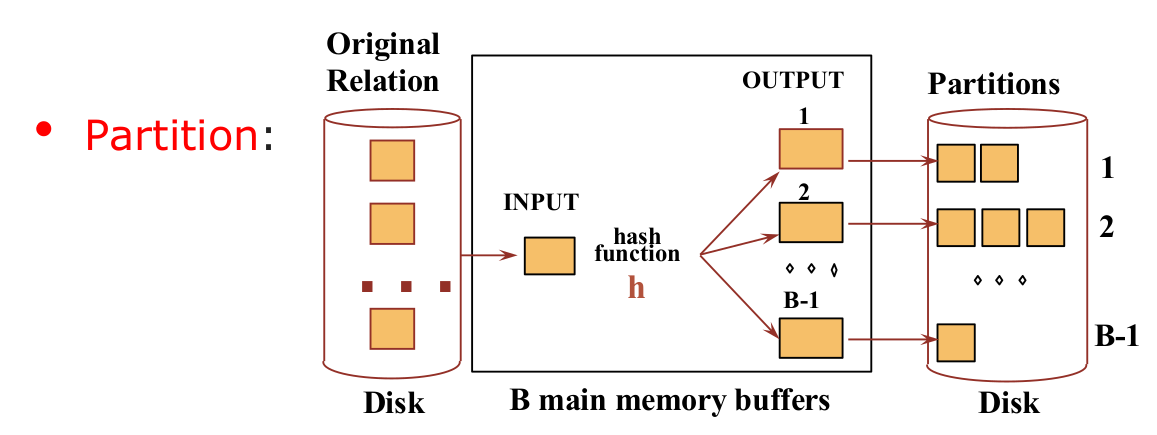
\includegraphics[scale=0.15]{graphics/hashing-partition.png}

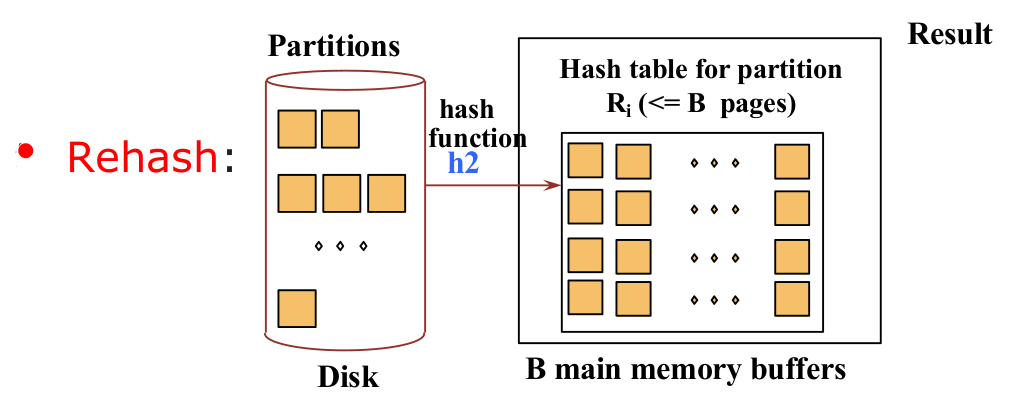
\includegraphics[scale=0.15]{graphics/hashing-rehash.png}

\paragraph{Duality of Sorting and Hashing}
\begin{itemize}
\item \textbf{Sorting:}
  \begin{itemize}
  \item physical division, logical combination
    \begin{itemize}
    \item Split followed by merge
    \item Recurse on merging
    \end{itemize}
  \item Sequential write (phase 1), random read (phase 2)
  \item Fan-in
  \item If pipelining and sqrt(N) < B < N, Total Cost = 3N
  \end{itemize}
\end{itemize}

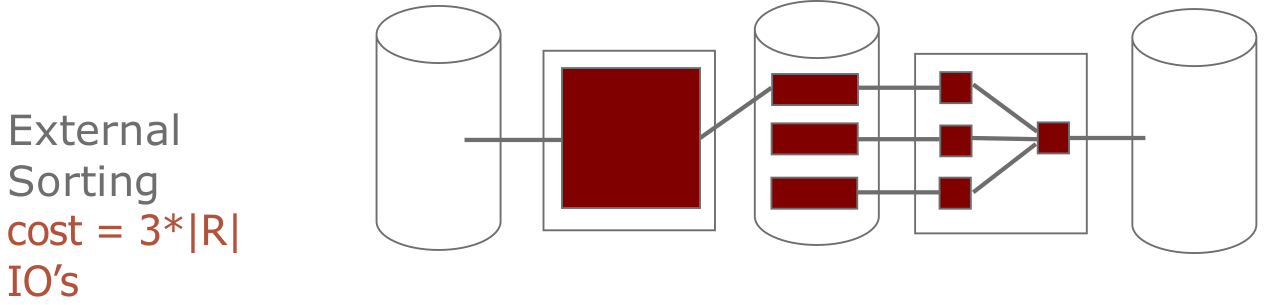
\includegraphics[scale=0.16]{graphics/external-sorting.png}

\begin{itemize}
\item \textbf{Hashing:}
  \begin{itemize}
  \item Logical division, physical combination
    \begin{itemize}
    \item partition followed by concatenate
    \item recurse on partitioning
    \end{itemize}
  \item random write (phase 1), sequential read (phase 2)
  \item Fan-out
  \item If pipelining and sqrt(N) < B < N, Total Cost = 3N
  \end{itemize}
\end{itemize}

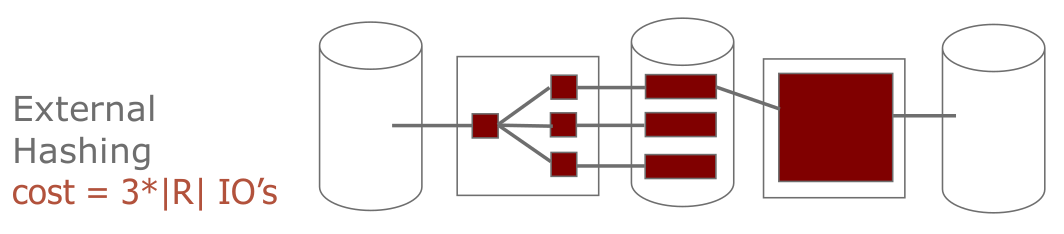
\includegraphics[scale=0.2]{graphics/external-hashing.png}

\paragraph{So which is better??}
\begin{itemize}
\item \textbf{Sorting pros:}
  \begin{itemize}
  \item Great if input already sorted (or almost sorted)
  \item Great if need output to be sorted anyway
  \item Not sensitive to ``data skew'' or ``bad'' hash functions
  \end{itemize}

\item \textbf{Hashing pros:}
  \begin{itemize}
  \item highly parallelizable
  \item Can exploit extra memory to reduce \# IOs with hybrid
    hashing
  \end{itemize}
\end{itemize}

\paragraph{Relational Operators: Joins}
\begin{itemize}
\item Joins are very common

  \begin{lstlisting}
    SELECT *
    FROM Reserves R1, Sailors S1
    WHERE R1.sid=S1.sid
  \end{lstlisting}
  
\end{itemize}

\paragraph{Simple Nested Loops Join}

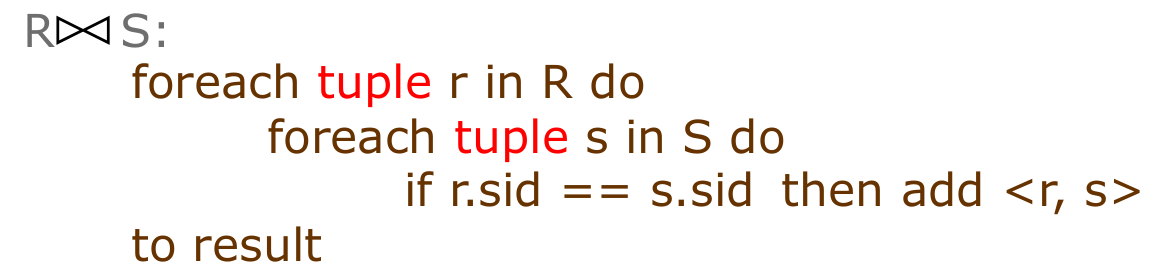
\includegraphics[scale=0.2]{graphics/nested-loop-join.png}

% LocalWords:  Unclustered unclustered superset goto ReHash Recurse
% LocalWords:  pipelining sqrt recurse parallelizable IOs
